\chapter{\textit{Document Planning}}
\label{cap:document_planning}

En la arquitectura presentada en el capítulo~\ref{cap:nlg_intro} mencionamos que el \emph{document planner} es el responsable de decidir que información comunicar (determinación de contenido) y como deberá estar estructurada esta información en el texto final (estructuración de documento). El \textit{document planner} será el encargado de que el documento final contenga toda la información requerida por el usuario y de que la misma se encuentre estructurada de una forma razonablemente coherente. El resultado de esta etapa será un \emph{document plan} en el cual se especificará qué contenido debe ser incluido en el texto final y de que forma deberá estar estructurado.


A continuación detallaremos las tareas que debe realizar el \textit{document planner}, describiremos brevemente la entrada y salida del mismo, definiremos como modelar los elementos informativos (estos serán elementos de nuestro \emph{document plan}) y finalmente estudiaremos las tareas puntuales.

%TODO

\section{Tareas del \textit{document planner}}
Como mencionamos anteriormente, el \textit{document planner} será el encargado de llevar a cabo las tareas de: \emph{determinación de contenido} y \emph{estructuración de documento}.

La \emph{determinación del contenido} es el nombre que se le da a la tarea de decidir y obtener la información que debemos comunicar en un texto. Este proceso generalmente involucra una o más procesos de \emph{selección}, \emph{resumen} y \emph{razonamiento con los datos} de entrada.

%TODO ejemplos?
\bigskip
\noindent
\textbf{Selección:} será el proceso encargado de recopilar un subconjunto de la información de entrada para luego poder ser comunicada al usuario final. El objetivo de éste será proveerle al usuario la información relevante requerida por el mismo.

\bigskip
\noindent
\textbf{Resumen:} será necesario cuando los datos de entrada son muy ``granulados'' para ser comunicados directamente o si la información relevante consiste alguna generalización o abstracción de los mismos.

\bigskip
\noindent
\textbf{Razonamiento con los datos:} resulta un caso general de las dos anteriores, generalmente mas sofisticado y más específico del dominio de aplicación. 

Para nuestro sistema de NLG será necesario realizar una tarea de \emph{selección} que recopile el conjunto de clases de prueba que debemos describir y luego procesaremos el resultado de la selección con el objetivo de, posteriormente, obtener mejores descripciones. En particular llevaremos a cabo dos tareas del tipo \emph{procesamiento con los datos}: \emph{eliminación de tautologías} y \emph{reducción de expresiones}. La primera nos permitirá filtrar expresiones que no añadirán información adicional a la descripción final y mientras que la \emph{eliminación de tautologías} será la encargada de simplificar algunas expresiones presentes en las clases de prueba lo que nos permitirá obtener descripciones mas concisas. En la sección \ref{cap:determinacion_contenido} retomaremos la \emph{determinación de contenido} estudiaremos mas en detalle las tareas mencionadas.

Finalmente, una vez seleccionada y procesada la información que debemos comunicar, será la etapa de \emph{estructuración de documento} la encargada de agrupar dicha información a fin de que el texto final resulte coherente y posea una estructura que le permita al lector interpretar con facilidad el contenido del mismo. Necesitaremos considerar como organizar y estructurar la información que tenemos que transmitir en el texto final con el fin de producir una descripción razonablemente fácil de leer y comprender. La \emph{estructuración de documento} deberá encargarse de aspectos estructurales a nivel del documento que deseamos producir, donde se contemplaran, por ejemplo, cuestiones como el orden en el que debe que ser comunicada la información, como estará agrupada la misma, etc. El resultado de la \emph{estructuración de documento} (y por lo tanto del \textit{document planner}), no será el texto final, sino que será una estructura intermedia de nuestro \textit{pipeline} que contendrá la información a comunicar en texto final agrupada convenientemente, llamada \emph{document plan}. 

En la próxima sección continuaremos definiremos detalladamente la entrada y salida del \textit{document planner} para luego estudiar en detalle las tareas a realizar durante la \emph{determinación de contenido} y finalmente veremos como estructurar nuestro documento. Esta estructura, el \emph{document plan}, será luego, la entrada del \emph{microplanner}.

\section{Entrada y salida del \textit{document planner}}
Como el document planner es el primer módulo de nuestro pipeline, la entrada de éste será la misma que la entrada de nuestro sistema. Reiter y Dale~\cite{reiter_dale} generalizan la entrada de un sistema de NLG  como una cuádrupla compuestas por los siguientes componentes:

\bigskip
\noindent
\textbf{Fuente de conocimiento:} Se refiere a las bases de datos e información del dominio de aplicación que nos proporcionará el contenido de la información que los textos generados deberán contener.
En nuestro caso la fuente de conocimiento estará compuesta por la especificación a testear, las clases de prueba generadas para ésta y las designaciones de la misma. 

\bigskip
\noindent
\textbf{Objetivo comunicacional:} Especifica el propósito que debe cumplir el sistema. En general esta compuesto por un ``tipo de objetivo'' y un parámetro.
En este trabajo tendremos solo un tipo de objetivo comunicacional: \emph{Describir(x)}, dónde el parámetro \emph{x} será un conjunto de identificadores de las clases de prueba a describir.

\bigskip
\noindent
\textbf{Modelo de usuario:} Provee información acerca del usuario (nivel de experiencia, preferencias, etc.). En nuestro caso el sistema se comportará de la misma forma independientemente del usuario, por lo que no tendremos en cuenta información del mismo.

\bigskip
\noindent
\textbf{Historial de discurso:} Consta de información sobre interacciones previas entre el usuario y el sistema. Este historial puede servir para algunos sistemas interactivos donde las interacciones anteriores con el usuario pueden resultar de utilidad. 

\bigskip
Como mencionamos anteriormente, la salida del document planner será un document plan que en nuestra arquitectura estará estructurado como un árbol, donde las hojas representarán el contenido y los nodos internos especificarán información estructural, por ejemplo sobre como debe agruparse la el contenido a comunicar. Para poder definir esta estructura, deberemos analizar primero como representar la información que necesitamos comunicar.

\section{Representación del dominio}


En los sistemas de NLG el texto generado se utiliza principalmente para transmitir información. Esta información será expresada generalmente en frases y palabras, pero estas  frases y palabras no son en si mismo la información; la información subyace estos constructores lingüísticos y es ``llevada'' por ellos. Nos deberemos concentrar entonces en como representar este conocimiento y como \textit{mapear} estas estructuras a una representación semántica. 

En esta sección definiremos los \emph{mensajes} que manipulará nuestro sistema. Llamamos \emph{mensajes}~\cite{reiter_dale} a los elementos informativos que conceptualizan la información que queremos comunicar; son paquetes de información que debe estar presente en el texto final. Estos estarán compuestos por elementos del dominio de aplicación.


El \emph{corpus de descripciones} (apéndice~\ref{ape:corpus}) resulta una buena fuente para estudiar el modelado del dominio y los tipos de \emph{mensajes} que necesitamos comunicar. Anteriormente, observamos en el \emph{corpus} la relación entre las frases pertenecientes a la información a comunicar y las expresiones Z de las clases de prueba generadas por Fastest. Observamos que estas clases de prueba están compuestas por una conjunción de predicados atómicos y que cada uno de estos predicados se corresponde con una oración en lenguaje natural dentro de la descripción de la clase de prueba. Podemos ver esta correspondencia en la figura \ref{fig:ej_test_desc}, donde las siguientes expresiones:

\medskip
\begin{enumerate}
  \item{$s? \in \dom st$}
  \item{$\dom st = \{ s? \}$}
\end{enumerate}

\medskip
\noindent
se encuentran, respectivamente, descritas por las siguientes frases:

\medskip
\begin{enumerate}
 \item{\emph{``El símbolo a buscar pertenece a los símbolos cargados en la tabla de símbolos.''}}
 \item{\emph{``El símbolo a buscar es el único elemento del conjunto formado por los símbolos cargados en la tabla de símbolos.''}}
\end{enumerate}

\bigskip
Por otro lado, también vimos que los textos correspondientes para cada uno de los predicados que componen una clase de prueba son independientes. Por lo que podríamos separar esta información en distintos mensajes facilitándole la tarea a las siguientes etapas de procesamiento. Es por esto que decidimos definir un único tipo de \emph{mensaje} para nuestro sistema: \emph{VerbalizacionExpresion} que representa, como su nombre lo indica, una verbalización de una expresión Z. Idealmente, tendremos un mensaje \emph{VerbalizacionExpresion} para cada uno de los predicado atómico pertenecientes a una clase de prueba.

En la figura~\ref{fig:ej_mensajes} podemos ver como quedarían definidos los mensajes para las expresiones mencionadas anteriormente.

\begin{figure}[H]
  	\centering
	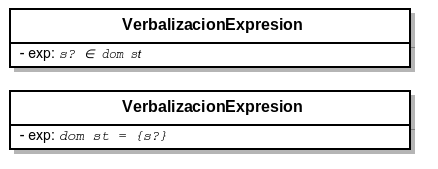
\includegraphics[scale=0.4]{img/mensajes.png}
	\caption{Mensajes a comunicar para el ejemplo de la figura~\ref{fig:ej_desc_lookup_sp_1}.}
  	\label{fig:ej_mensajes}
\end{figure}

Vale la pena aclarar que en nuestro caso, los datos con los que trabajamos resultan esquemas Z de las clases de prueba, por lo que ya se encuentran modelados de antemano y no fue necesario realizar un nuevo modelo del dominio.
 

\section{Determinación del contenido}
\label{cap:determinacion_contenido}

Como mencionamos anteriormente, en la \emph{determinación de contenido} se suelen llevar a cabo una o mas tareas de \emph{selección}, \emph{resumen} y \emph{razonamiento con los datos}. En la figura                     \ref{fig:tareas_determinacion_contenido} podemos observar estas tareas y posteriormente veremos cada una de ellas mas detalladamente.

Podemos observar en la figura \ref{fig:tareas_determinacion_contenido} las tres tareas que nuestro sistema deber

\begin{figure}[H]
  	\centering
	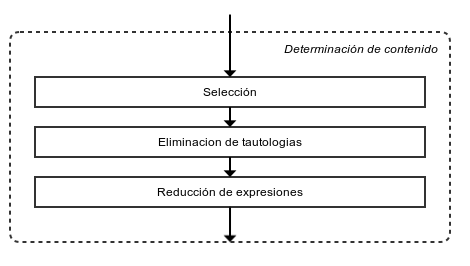
\includegraphics[scale=0.4]{img/tareas_determinacion_contenido.png}
	\caption{Tareas determinación de contenido.}
  	\label{fig:tareas_determinacion_contenido}
\end{figure}



\subsection*{Selección}
Como vimos en la sección anterior, nuestro sistema de NLG deberá ser capaz de producir descripciones para un subconjunto de clases de prueba del total de las clases generadas por \emph{Fastest} para una especificación. Es decir, el usuario podría solicitarle a nuestro sistema la generación de descripciones para una, un grupo o todas las clases de pruebas incluidas en la especificación y el sistema debería generar descripciones únicamente para las clases de prueba indicadas. Es por esto que deberemos realizar una \emph{selección de la información} que tendrá luego que ser incluida dentro del \textit{document plan} a fin de ser comunicada, posteriormente, en el texto final.

Como mencionamos previamente, la tarea de \emph{selección de información} para nuestro trabajo se resumirá a la búsqueda y filtrado de las clases de prueba indicadas por el usuario dentro de todo el conjunto de clases de prueba que forma parte de la entrada del sistema. Por ejemplo, si deseamos generar una descripción para la clase de prueba \emph{LookUp\_SP\_1} de la figura~\ref{fig:ej_tcl_lookup}, la misión de de esta tarea será la de identificar y seleccionar la clase \emph{LookUp\_SP\_1} entre todas las generadas por \emph{Fastest} que formarán parte de los datos de entrada de nuestro sistema de NLG.

%TODO agregar grafico aca para ejemplificar?

A continuación veremos como podemos mejorar las descripciones de nuestro sistema realizando algunos procesamientos sobre la información seleccionada previo a la construcción del \textit{document plan}. En particular veremos dos tareas que podríamos enmarcar dentro del \emph{razonamiento con los datos}, la \emph{eliminación de tautologías} y la \emph{reducción de expresiones}. 

% que eliminando tautologías de los esquemas de clase de prueba y realizando algunas reducciones simples sobre las expresiones de los mismos podremos, posteriormente, obtener mejores descripciones.

\subsection*{Eliminación de tautologías}
Como mencionamos anteriormente, todas las clases de prueba incluidas en el \emph{corpus} fueron generadas utilizando \emph{Fastest 1.6}. Hemos observado que en ciertos casos, esta herramienta genera clases de prueba como la que podemos ver, por ejemplo, en la figura \ref{fig:ej_update_sp_4}.

\begin{figure}[H]
  \centering
  \begin{schema}{Update\_ SP\_ 4}\\
   st : SYM \pfun VAL \\
   s? : SYM \\
   v? : VAL 
  \where
   st \neq \{ \} \\
   \{ s? \mapsto v? \} \neq \{ \} \\
   \dom st = \dom \{ s? \mapsto v? \}
  \end{schema}
  \caption{Clase de prueba para operación Update (pág.~\pageref{fig:spec_symbol_table}).}
  \label{fig:ej_update_sp_4}
\end{figure}

Podemos observar en este caso, que la siguiente expresión del ejemplo anterior:

\begin{figure}[H]
  \centering
  $\{ s? \mapsto v? \} \neq \{ \}$ 
\end{figure}

\noindent
no aporta información relevante para el usuario, de hecho esta expresión no agrega ninguna restricción para el caso de prueba ya que será siempre verdadera y si intentáramos describir este predicado, terminaríamos con un texto parecido al siguiente:

\begin{figure}[H]
  \centering
  \emph{``el conjunto formado por el par de el símbolo a actualizar y el nuevo valor, es distinto al conjunto vacío''}
\end{figure}

\noindent
que además de resultar algo difícil de interpretar, no aporta nada al objetivo comunicacional.

En la versión de \emph{Fastest} utilizada observamos que sólo se introducían tautologías similares a la del ejemplo anterior. Puntualmente sólo vimos que ocurría con predicados del tipo:

\begin{figure}[H]
  \centering
  $\{ a, b, ... , n \} \neq \{ \}$ 
\end{figure}



Por lo tanto, obtendremos descripciones mas claras si no intentamos comunicar esta clase de predicados. Para nuestro sistema deberá filtrar las tautologías presentes en las clases de prueba y no incluirlas dentro del \emph{document plan}.

%TODO
%1- como determino tautologias
%2- casos
%3- que simplifico/reduzco
%4- no dijimos que eran atómicos?
%hablo de todo esto en el capitulo del corpus?



\subsection*{Reducción de expresiones}

%TODO en algun lado decir que hay predicados que no son atomicos y de ellos nos encargaremos en esta secciòn

%TODO cierre capítulo


Una vez seleccionada y procesada la información necesaria será ésta etapa la encargada de construir los mensajes introducidos en la sección anterior, que luego formarán parte de nuestro \emph{document plan}.

Para nuestro trabajo, la tarea de \emph{selección} 

Luego de la \emph{selección}, nuestro sistema deberá procesar los datos de entrada con el fin de obtener mejores descripciones. Hemos observado\footnote{Análisis en base a clases de prueba generados utilizando \emph{Fastest 1.6}} que trabajando ciertas expresiones en las clases de prueba podemos mejorar considerablemente los textos producidos. Veamos por ejemplo la figura~\ref{fig:ej_update_sp_4} donde se muestra una clase de prueba generada con \emph{Fastest} en la que se pueden ver dos problemas que abordaremos en esta etapa.

\begin{figure}[H]
  \centering
  \begin{schema}{Update\_ SP\_ 4}\\
   st : SYM \pfun VAL \\
   s? : SYM \\
   v? : VAL 
  \where
   st \neq \{ \} \\
   \{ s? \mapsto v? \} \neq \{ \} \\
   \dom st = \dom \{ s? \mapsto v? \}
  \end{schema}
  \caption{Clase de prueba para operación Update (pág.~\pageref{fig:spec_symbol_table}).}
  \label{fig:ej_update_sp_4}
\end{figure}







\noindent
que además de poder resultar algo difícil de interpretar, no aportaría nada al objetivo comunicacional.

Por otro lado, en un primer intento por describir automáticamente la expresión:

\begin{figure}[H]
  \centering
  $\dom st = \dom \{ s? \mapsto v? \}$ 
\end{figure}

\noindent
podríamos describirla como\footnote{Esta descripción sería la generada utilizando el sistema de reglas propuesto en el capítulo~\ref{TODO} si no trabajamos la expresión en una etapa previa.}:

\begin{figure}[H]
  \emph{``el conjunto de símbolos cargados en la tabla es igual a el dominio del par formado por el símbolo a actualiza y el nuevo valor''}
\end{figure}

Veamos que es posible simplificar notablemente esta descripción si antes trabajamos la expresión anterior, que resulta equivalente a:

\begin{figure}[H]
  \centering
  $\dom st = \{s?\}$ 
\end{figure}

\noindent
que luego podríamos describir como:

\begin{figure}[H]
  \emph{``el símbolo a actualizar es el único elemento en la tabla de símbolos cargados''}
\end{figure}

En conclusión, el procesamiento que nos proponemos a realizar en esta etapa tendrá dos objetivos:
\begin{enumerate}
  \item Eliminar tautologías de las expresiones que forman parte de las clases de prueba seleccionadas.
  \item Realizar algunas simplificaciones o reducciones triviales.
\end{enumerate}

\bigskip
Una vez seleccionada y procesada la información deberemos construir los \emph{mensajes} (\emph{VerbalizacionExpresion}) que luego formarán parte del \emph{document plan} desarrollado en el siguiente capítulo.

\section{Estructuración del documento}
\label{sec:document_structure}

Como dijimos antes, el texto generado no podrá ser una colección al azar de frases y palabras. Deberá tener coherencia y poseer una estructura que le permita al lector interpretar con facilidad el contenido del mismo.
Necesitaremos considerar como organizar y estructurar la información que debemos comunicar con el fin de producir un texto razonablemente fácil de leer y comprender.

%~\footnote{Las decisiones sobre como debe estar ordenado y agrupado el documento final son resultado del análisis del \emph{corpus} de descripciones.}
En esta tarea nos concentraremos en construir una estructura que contenga los \emph{mensajes} seleccionados en la etapa de \emph{determinación de contenido}; estableciendo el agrupamiento y ordenamiento de los mismos. Esta estructura deberá caracterizar la disposición de los elementos pertenecientes a los textos recopilados en el \emph{corpus}. 

Tomando el \emph{corpus} de descripciones como una especificación de los documentos que debemos generar podemos observar que estos documentos poseen una estructura bastante simple y rígida a la vez. Estos documentos deben estar formados por una secuencia de descripciones para las clases de prueba indicadas por el usuario, ordenadas alfabéticamente según el nombre de la clase de prueba. A su vez, cada una de estas descripciones deberá agrupar las verbalizaciones de las expresiones seleccionadas en la etapa de \emph{determinación de contenido}, ordenadas de la misma forma en la que aparecen en el esquema de la clase de prueba en cuestión. En la figura~\ref{fig:png_document_plan} podemos observar una representación abstracta de la estructura propuesta para modelar el documento.

\begin{figure}[H]
  	\centering
	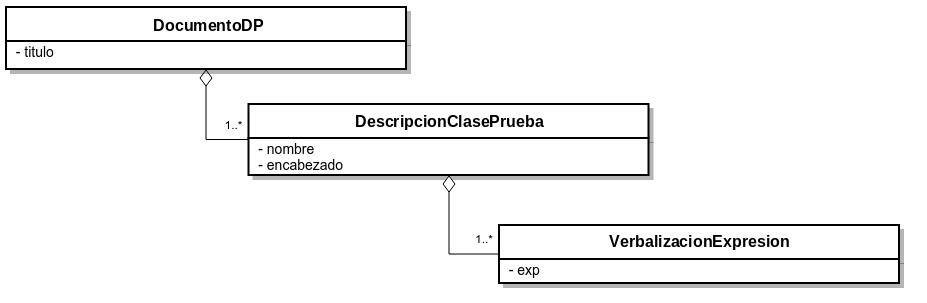
\includegraphics[scale=0.4]{img/document_plan.png}
	\caption{Document plan.}
  	\label{fig:png_document_plan}
\end{figure}

Llamaremos \emph{DocumentoDP} a la raíz de nuestro \emph{document plan}, \emph{DocumentoDP} contendrá a su vez una lista ordenada de las descripciones de las clases de prueba (\emph{DescripcionClasePrueba}) que debemos incluir en el texto final. El elemento \emph{DescripcionClasePrueba} representa el texto a generar para una clase de prueba (por ejemplo el texto de la figura~\ref{fig:ej_lookup_sp_1}) y tendremos uno de estos elementos por cada clase de prueba indicada por el usuario. Finalmente los mensajes seleccionados en la etapa anterior formarán se encontrarán agrupados en la \emph{DescripcionClasePrueba} correspondiente. Podemos ver en la figura~\ref{fig:png_document_plan_ej} un ejemplo del document plan para la descripción de la clase de prueba \emph{LookUp\_SP\_1} introducida anteriormente. 

\begin{figure}[H]
  	\centering
	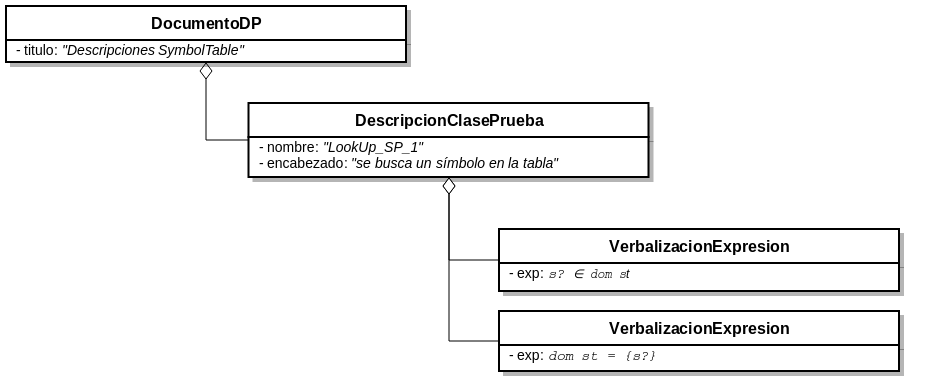
\includegraphics[scale=0.4]{img/document_plan_ej.png}
	\caption{Document plan correspondiente al texto de la figura~\ref{fig:ej_lookup_sp_1}.}
  	\label{fig:png_document_plan_ej}
\end{figure}


